%\documentclass[12pt, answers]{exam}
\documentclass[12pt]{exam}
\usepackage[utf8]{inputenc}

\usepackage[margin=1in]{geometry}
\usepackage{amsmath,amssymb}
\usepackage{multicol}
\usepackage[]{graphicx}
\usepackage[]{bm}
\usepackage[]{nicefrac}
\usepackage[]{xcolor}

\DeclareMathOperator*{\argmin}{argmin}
\DeclareMathAlphabet{\mathcal}{OMS}{cmsy}{m}{n}
\DeclareMathAlphabet\mathbfcal{OMS}{cmsy}{b}{n}
\DeclareMathOperator*{\minimize}{minimize~}
\DeclareMathOperator*{\maximize}{maximize~}
\DeclareMathOperator*{\subjectto}{subject~to~}


\newcommand{\class}{Mathematics for Engineers}
\newcommand{\term}{Master 1}
\newcommand{\examnum}{Exam}
\newcommand{\examdate}{2021-2022}
\newcommand{\timelimit}{120 Minutes}

\pagestyle{head}
\firstpageheader{}{}{}
\runningheader{\class}{\examnum\ - Page \thepage\ of \numpages}{\examdate}
\runningheadrule

\usepackage[]{tikz}

\begin{document}

\noindent
\begin{tabular*}{\textwidth}{l @{\extracolsep{\fill}} r @{\extracolsep{6pt}} l}
  \textbf{\class} \\%& \textbf{Nom -- Prénom:} & \makebox[2in]{\hrulefill}\\
  % \textbf{\term} &&\\
  \textbf{\examnum} &&\\
  \textbf{\examdate} && \\
  % \textbf{Time Limit: \timelimit} & Teaching Assistant & \makebox[2in]{\hrulefill}
  \textbf{Time limit: \timelimit} %&&
\end{tabular*}\\
\rule[2ex]{\textwidth}{2pt}

This exam contains \numpages\ pages (including this cover page) and \numquestions\ exercises. \\

%% \begin{center}
%%   Barême\\
%%   \bigskip
%%   \addpoints
%%   \gradetable[v][questions]
%% \end{center}

\noindent
\rule[2ex]{\textwidth}{2pt}

\begin{questions}

  %%%%%
  %%%%%
  %%%%%

  \question \textbf{Input-Output relation}
  \noaddpoints

  Consider the discrete-time linear dynamical system
  %
  \[
  \begin{aligned}
    \bm{x}_{k+1} & = \bm{Ax}_k + \bm{Bu}_k \\
    \bm{y}_k & = \bm{Cx}_k + \bm{Du}_k.
  \end{aligned}
  \]
  %
  Find the matrix $\bm{G}$ such that
  %
  \[
  \begin{bmatrix}
    \bm{y}_0 \\ \bm{y}_1 \\ \bm{y}_2 \\ \vdots \\ \bm{y}_{n-1} \\ \bm{y}_n
  \end{bmatrix}
  =
  \bm{G}
  \begin{bmatrix}
    \bm{x}_0 \\
    \bm{u}_0 \\
    \bm{u}_1 \\
    \vdots \\
    \bm{u}_{n-1} \\
    \bm{u}_n
  \end{bmatrix}.
  \]
  %
  The matrix $\bm{G}$ shows  how the output at time $k = 0, \cdots, n$ depends on the initial state $\bm{x}_0$ and the sequence of inputs $\bm{u}_0, \cdots, \bm{u}_n$.

  %%%%%
  %%%%%
  %%%%%

  \begin{solution}
    {\color{blue}
      \ldots
    }
  \end{solution}




  %%%%%
  %%%%%
  %%%%%

  \question \textbf{Estimating with known input norm}

  We consider a standard estimation setup
  %
  \[
  \bm{y} = \bm{Ax} + \bm{v}
  \]
  %
  where $\bm{A} \in \mathbb{R}^{m \times n}$ is a full rank skinny matrix, $\bm{x} \in \mathbb{R}^n$ is the vector we wish to estimte and $\bm{v}$ are small measurement errors.
  In this problem, we add a more piece of prior information : we known that
  %
  \[
  \| \bm{x} \|_2 = 1,
  \]
  %
  i.e. we know ahead of time that the vector we are estimating has norm one.
  This might occur in a communication system where the transmitted signal power is known to be equal to one.
  We will assume furthemore that the norm of the least-squares approximate solution $\| \left( \bm{A}^T \bm{A} \right)^{-1} \bm{A}^T \bm{y} \|_2 > 1$.

  Explain clearly how would you find the best estimate of $\bm{x}$ taking into account the prior knowledge that $\| \bm{x} \|_2 = 1$.
  Explain how you would compute your estimate $\hat{\bm{x}}$ given $\bm{A}$ and $\bm{y}$. (\underline{Hint :} you'll need to introduce a Lagrange multiplier.)

  %%%
  %%%
  %%%

  \begin{solution}
    {\color{blue}
      \ldots
    }
  \end{solution}




  %%%%%
  %%%%%
  %%%%%

  \question \textbf{Interconnection of linear systems}

  often a linear system is described in terms of a block diagram showing the interconnections between components or subsystems which are themselves linear systems.
  In this problem, you consider the specific interconnection shown in figure~\ref{fig: interconnection of linear systems}.

  \begin{figure}
    \centering
    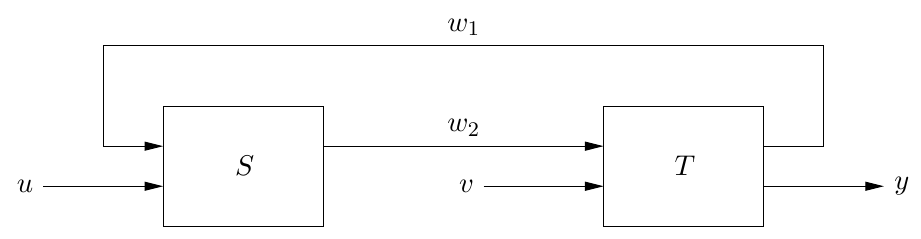
\includegraphics[width=.8\textwidth]{lti_system.png}
    \caption{
      Schematic of the system considered.
    }
    \label{fig: interconnection of linear systems}
  \end{figure}

  Here, there are two subsystems $S$ and $T$.
  Subsystem $S$ is characterized by
  %
  \[
  \begin{aligned}
    \dot{\bm{x}} & = \bm{Ax} + \bm{B}_1 \bm{u} + \bm{B}_2 \bm{w}_1 \\
    \bm{w}_2 & = \bm{Cx} + \bm{D}_1 \bm{u} + \bm{D}_2 \bm{w}_1
  \end{aligned}
  \]
  %
  and subsystem $T$ is characterized by
  %
  \[
  \begin{aligned}
    \dot{\bm{z}} & = \bm{Fz} + \bm{G}_1 \bm{v} + \bm{G}_2 \bm{w}_2 \\
    \bm{w}_1 & = \bm{H}_1 \bm{z} \\
    \bm{y} & = \bm{H}_2 \bm{z} + \bm{Jw}_2.
  \end{aligned}
  \]
  %
  We don't specify the dimensions of the signals or matrices here and so you can assume that all matrices are the correct (i.e. compatible) dimensions.

  Express the overall system as a single linear dynamical system with input, state and output given by
  %
  \[
  \begin{bmatrix}
    \bm{u} \\ \bm{v}
  \end{bmatrix},
  \quad
  \begin{bmatrix}
    \bm{x} \\ \bm{z}
  \end{bmatrix},
  \quad
  \text{and}
  \quad
  \bm{y},
  \]
  %
  respectively.
  Be sure to explicitly give the input, dynamics, output and feedthrough matrices of the overall system.

  %%%%%
  %%%%%
  %%%%%

  \begin{solution}
    {\color{blue}
      \ldots
    }
  \end{solution}




  %%%%%
  %%%%%
  %%%%%

  \question \textbf{A method for rapidly driving the state to zero}

  Consider the discrete-time linear dynamical system
  %
  \[
  \bm{x}_{k+1} = \bm{Ax}_k + \bm{Bu}_k
  \]
  %
  where $\bm{A} \in \mathbb{R}^{n \times n}$ and $\bm{B} \in \mathbb{R}^{n \times k}$ are full rank with $k \leq n$.
  The goal is to choose an input $\bm{u}$ that causes $\bm{x}_k$ to converge to zero as $t \to \infty$.
  An egineer argues that this scheme will work well since the norm of the state is made as small as possible at every step.
  In this problem you will analyze this scheme.

  \begin{parts}
    \part Find an explicit expression for the proposed input $\bm{u}_k$ as a function of $\bm{x}_k$, $\bm{A}$ and $\bm{B}$.

    \part Now consider the linear dynamical system $\bm{x}_{k+1} = \bm{Ax}_k + \bm{Bu}_k$ with $\bm{u}_k$ given by the proposed scheme (i.e. as found in the previous question).
    Show that $\bm{x}$ statisfies an autonomous linear dynamical system equation $\bm{x}_{k+1} = \bm{Fx}_k$.
    Express this matrix $\bm{F}$ explicitely in terms of $\bm{A}$ and $\bm{B}$.
  \end{parts}

  %%%%%
  %%%%%
  %%%%%

  \begin{solution}
    {\color{blue}
      \ldots
    }
  \end{solution}





  %%%%%
  %%%%%
  %%%%%

  \question \textbf{Energy storage efficiency in a linear dynamical system}

  Consider the SISO discrete-time linear dynamical system
  %
  \[
  \begin{aligned}
    \bm{x}_{k+1} & = \bm{Ax}_k + \bm{B}u_k \\
    y_k & = \bm{Cx}_k,
  \end{aligned}
  \]
  %
  with $y_k$ and $u_k \in \mathbb{R}$.
  The initial state is $\bm{x}_0 = \bm{0}$.
  We apply an input sequence $u_0, \cdots, u_{n-1}$ and are interested in the output over the next $n$ samples, i.e. $y_n, \cdots, y_{2n-1}$.
  We assume furthermore that $u_k = 0$ for $k \geq n$.

  \begin{parts}
    \part Give the expression of the matrix $\bm{G}$ such that
    %
    \[
    \begin{bmatrix}
      y_n \\ y_{n+1} \\ \vdots \\ y_{2n-2} \\ y_{2n-1}
    \end{bmatrix}
    =
    \bm{G}
    \begin{bmatrix}
      u_0 \\ u_1 \\ \vdots \\ u_{n-2} \\ u_{n-1}
    \end{bmatrix}.
    \]

    \part We define the \emph{input energy} as
    %
    \[
    \mathcal{E}_{\text{in}} = \sum_{k=0}^{n-1} u_k^2
    \]
    %
    and similarly the output energy is defined as
    %
    \[
    \mathcal{E}_{\text{out}} = \sum_{k=n}^{2n-1} y_k^2.
    \]
    %
    We wish to find the input sequence $u_0, \cdots, u_{n-1}$ maximizing the ratio of output energy to input energy.
    Formulate the corresponding optimization problem and explain how one could obtain the optimal solution.

  \end{parts}
\end{questions}

\end{document}
